\chapter{Background}
\label{ch:background}



\graphicspath{{snoga/}}
%\section{Computational Phylogenetics}
Computational phylogenetics deals with the design and application of computational tools and techniques to conduct necessary analyses related to phylogeny estimation. The primary aim is to reconstruct a most probable hypothesis about the evolutionary ancestry of a set of taxa (i.e., genes, species, etc.). Here we briefly describe the preliminary concepts involved in computational phylogenetics. 
%\begin{comment}
\section{Phylogeny}
Phylogeny refers to the evolutionary relationships among a set of entities such as species, genes, etc popularly represented as a tree known as phylogenetic tree. The entities under consideration are generally referred to as taxa. Each such taxon is placed as a leaf node in a phylogenetic tree and the tree topology represents the evolutionary history. The  internal nodes of the tree represent hypothetical ancestral taxa from which the present day taxa evolved. These ancestral taxa are believed to have existed in the past, but has become extinct. Notably, a tree $T$ is a connected acyclic graph with a set of vertices $V$ and a set of edges $E$. An edge $e = (u, v) \in E$ represents an evolutionary relationship between the two taxa represented by the vertices $u$ and $v$. 

\begin{figure}[!htbp]
\centering
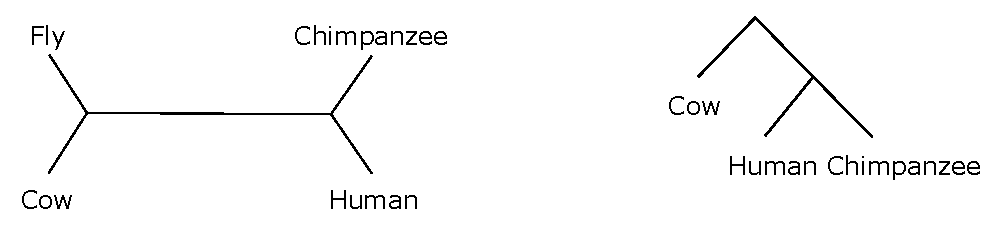
\includegraphics[width=0.9\textwidth]{Figure/outgroup.eps}
\caption{A phylogenetic tree relating four species: human, chimpanzee, gorilla and orangutan. }
\label{fig:outgroup}
\end{figure}

Fig.~\ref{fig:outgroup} shows an example phylogenetic tree among four species: human, chimpanzee, gorilla and orangutan. This evolutionary tree depicts that human and chimpanzee share a common ancestor. As such, we consider humans to be more closely related to chimpanzees than they are to gorillas and orangutans.
%\end{comment}
%\subsubsection{Rooted and unrooted trees} 
In a rooted phylogenetic tree (left part of Fig.~\ref{fig:outgroup}), one vertex $r \in V$ is designated as the root of the tree whereas there is no such designated vertex in an unrooted tree (right part of Fig.~\ref{fig:outgroup}). True evolutionary histories are better represented by a rooted tree. However, identifying the root of an estimated phylogenetic tree is generally a difficult task.

\subsection{Phylogeny Estimation}

\subsection{Evaluation of Phylogeny Estimation Methods}\label{sec:phyPerf}
The performance of a species tree estimation is evaluated by comparing its output tree to the ground truth (i.e., true species tree provided with the simulated dataset) using False Negative (FN) rate also known as the missing branch rate. FN rate actually expresses (in percentage) the fraction of edges that exist in the latter (i.e., in true tree) but are absent in the former (i.e., in the estimated one). Clearly, the smaller the
value of FN rate, the more desirable it is. Although there are two more common tree error measures (False Positive (FP rate) and Robinson-Foulds (RF) rate), all of them are identical when true and estimated trees are binary. In this thesis, we worked with binary trees only.

\subsection{Discordance between Gene and Species Phylogeny}\index{Gene tree discordance}
We now discuss the issue of discordance between a gene tree and species tree and the reasons behind it. A species tree represents the evolutionary history among a set of species via the process of speciation. On the contrary, a gene tree represents the evolution of a particular ``gene" within a group of species. When species are split by speciation, the gene copies within species are also split into separate lineages of descent.  Within each such lineage, the gene trees continue branching and descending through time. Thus, the gene trees are contained within the branches of the species trees~\cite{maddison1997gene}.
However, when gene copies are sampled from various species, the gene tree relating these copies might disagree with the species phylogeny. Fig.~\ref{fig:discordance} shows an example of discordance between a species tree and a gene tree. Here, species $B$ and $C$ are ``sister" species. However, in the gene lineage, $C$ is closer to $D$ than $B$. This discord can arise from the horizontal transfer, incomplete lineage sorting, and gene duplication and extinction~\cite{maddison1997gene}. 

\begin{figure}[!tb]
	\centering
	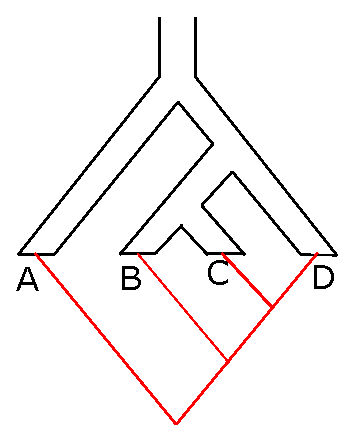
\includegraphics[width=0.33\textwidth]{Figure/discordance.eps}
	\caption{Gene tree-species tree discordance. A species tree (given in block diagram) and a gene tree (given in line diagram) on the same set $\{A,B,C,D\}$ of taxa with different topologies.}
	\label{fig:discordance}
\end{figure}



\subsubsection{Incomplete Lineage Sorting}\index{Incomplete lineage sorting (ILS)}

%Incomplete lineage sorting (ILS) refers to the failure of two gene lineages to coalesce at their speciation point. Also known as deep coalescence, this process is best understood under the multi-species coalescent (MSC) model~\cite{degnan2006discordance, degnan2005gene}. This model explains the evolutionary process by going backward in time and connecting gene lineages to a common ancestor through a process of ``coalescence" of lineage pairs. This is explained with an example in the Appendix.
%\section{Incomplete Lineage Sorting}%\index{Incomplete lineage sorting (ILS)}

Incomplete lineage sorting (ILS) refers to the failure of two gene lineages to coalesce at their speciation point. Also known as deep coalescence, this process is best understood under the coalescent model~\cite{degnan2006discordance, degnan2005gene}. This model explains evolutionary process by going backwards in time and connecting gene lineages to a common ancestor through a process of ``coalescence" of lineage pairs. In this model, each species is treated as a population of individuals, having a pair of alleles for each gene. The present day variants of a gene (known as alleles) are then traced back in time across successive generations by following the ancestral alleles in the previous generation from which this given alleles evolved. Eventually a point is reached where two alleles coalesce (i.e., they find a common ancestor). The multi-species coalescent (MSC) model is the extension of this general coalescent framework where multiple randomly mating populations corresponding to multiple species are present.
%, nei1987molecular, tajima1983evolutionary, takahata1989gene
\begin{figure}[!tb]
	\centering
	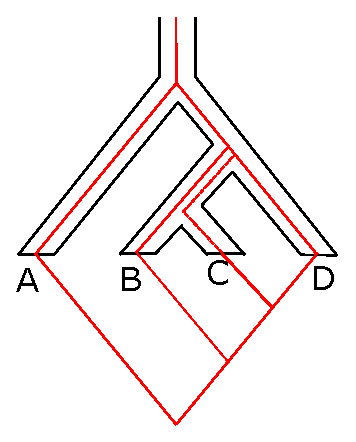
\includegraphics[width=0.33\textwidth]{Figure/ils.eps}
	\caption{Example of gene tree-species tree discordance due to incomplete lineage sorting. Going back in time, the gene copies within species $B$ and $C$ first meet at their corresponding speciation point, but fail to coalesce. Both the lineages (dashed and solid black lines) exist on deeper ancestral branch. The gene from $C$ first coalesces with the gene from species $D$, and subsequently with the gene from $B$.
	}
	\label{fig:ils}
\end{figure}
Under the MSC model, ILS can be a source of gene tree discordance, as the common ancestry of gene copies at a single locus can extend deeper than speciation events. The larger the effective population size and the shorter the branch length of the evolutionary tree, the greater the chance of ILS or deep coalescence to occur~\cite{maddison1997gene}.

Figure~\ref{fig:ils} shows an example of discordance due to ILS. The gene copies within species $B$ and $C$ first meet at their corresponding speciation point as we go back in time. The speciation point is the most recent common ancestor of species $B$ and $C$. However, the gene copies fail to coalesce here. Both of these copies go further back in time, resulting in two gene lineages on deeper ancestral branch. The extra lineage is shown by the dashed red lines in Figure~\ref{fig:ils}. Then the gene from $C$ first coalesces with the gene from species $D$, and subsequently with the gene from $B$.

\begin{comment}

\subsubsection{Quartet Score}
The quartet score~\cite{mirarab2014astral} measures the similarity between a candidate species tree $T$ and the input gene trees, and is computed as follows. Each input gene tree is decomposed into its induced set of quartet trees (i.e., unrooted trees formed by picking four leaves). The quartet support score of a given candidate species tree $T$ is the total, overall the input gene trees, of the number of induced quartet trees that $T$ agrees with. This score is maximized by ASTRAL to estimate the species tree. 

\subsubsection{Triplet Score}
The triplet score~\cite{islam2019stelar}, similar to quartet score, counts the number of induced triplet trees (i.e., rooted trees formed by picking three leaves) of the candidate species tree that agrees with the input gene trees. This criterion is maximized by STELAR. 

\subsubsection{Pseudo-likelihood}
It measures the likelihood of a candidate species tree given the triplet distribution of the input gene trees and maximized by MP-EST~\cite{mpest} as an estimator of the species tree.
\end{comment}

\subsubsection{Statistical consistency}\index{Statistical consistency}

A species tree reconstruction method is said to be statistically consistent under a particular model of evolution if the probability of returning the true species tree converges to one as the amount of data increases. Let the set of genes in a study be $\mathcal{G} = \{g_1, g_2, \dots, g_M\}$. Let $s_i$ be the number of sites in $g_i$ ($1 \leq i \leq M$). Then A species tree estimation method is statistically consistent if the estimated species tree converges to the true species tree as $M \rightarrow \infty$, $\underset{1 \leq i \leq M}{s_i} \rightarrow \infty$.


\subsubsection{Optimization criteria for species tree estimation}
Various criteria are statistically consistent estimators of the true species tree under the MSC model. Each of them measures how well a candidate species tree can summarize the input gene trees. Three examples are as follows:
\begin{itemize}
	\item Quartet score \cite{mirarab2014astral}: The quartet score of a given candidate species tree $T$ is the total, across all the input gene trees, of the number of induced quartet trees that $T$ agrees with. This score is maximized by ASTRAL to estimate the species tree.
	\item Triplet score \cite{islam2019stelar}: Similar to quartet score, it counts the number of induced triplet trees (i.e., rooted trees formed by picking three leaves) of the candidate species tree that agrees with the input gene trees.
	\item Pseudo-likelihood \cite{mpest}: It measures the likelihood of a candidate species tree given the triplet distribution of the input gene trees.
\end{itemize}


\section{Multiple Sequence Alignment}
Multiple sequence alignment (MSA) task seeks to arrange three or more nucleotide/protein sequences to infer homology, considering various biological phenomena (i.e., evolutionary history, 3D structure etc.). The output is a matrix in which the input nucleotide/protein sequences are the rows and each column (i.e., site) has characters which are homologous which means all those letters descend from the same letter of a common ancestor). The aligned sequences reflect historical substitution, insertion and deletion of genetic materials which are represented as gaps. Accurately recovering these properties through MSA is necessary to accomplish a biological objective such as inferring the evolutionary history relating the sequences known as phylogenetic trees. While computing MSAs, various computational methods and criteria are used to make hypotheses about homology. But the goal of MSA is entirely biological. Figure~\ref{fig:msa_io} illustrates this problem using an example where four hypothetical protein sequences are to be aligned by placing ``necessary'' gaps. %In this work, we focus on the MSA tasks in the context of phylogeny estimation which usually functions in two steps. Firstly, the given sequences are aligned using an MSA tool, thereafter a phylogenetic tree is inferred on obtained alignment. The goodness of estimated phylogenetic trees largely rely on the properties of the corresponding alignment. Thus, choosing the ``most appropriate'' MSA method  is important in the phylogenetic context.

\begin{figure}[!htbp]
	\centering
	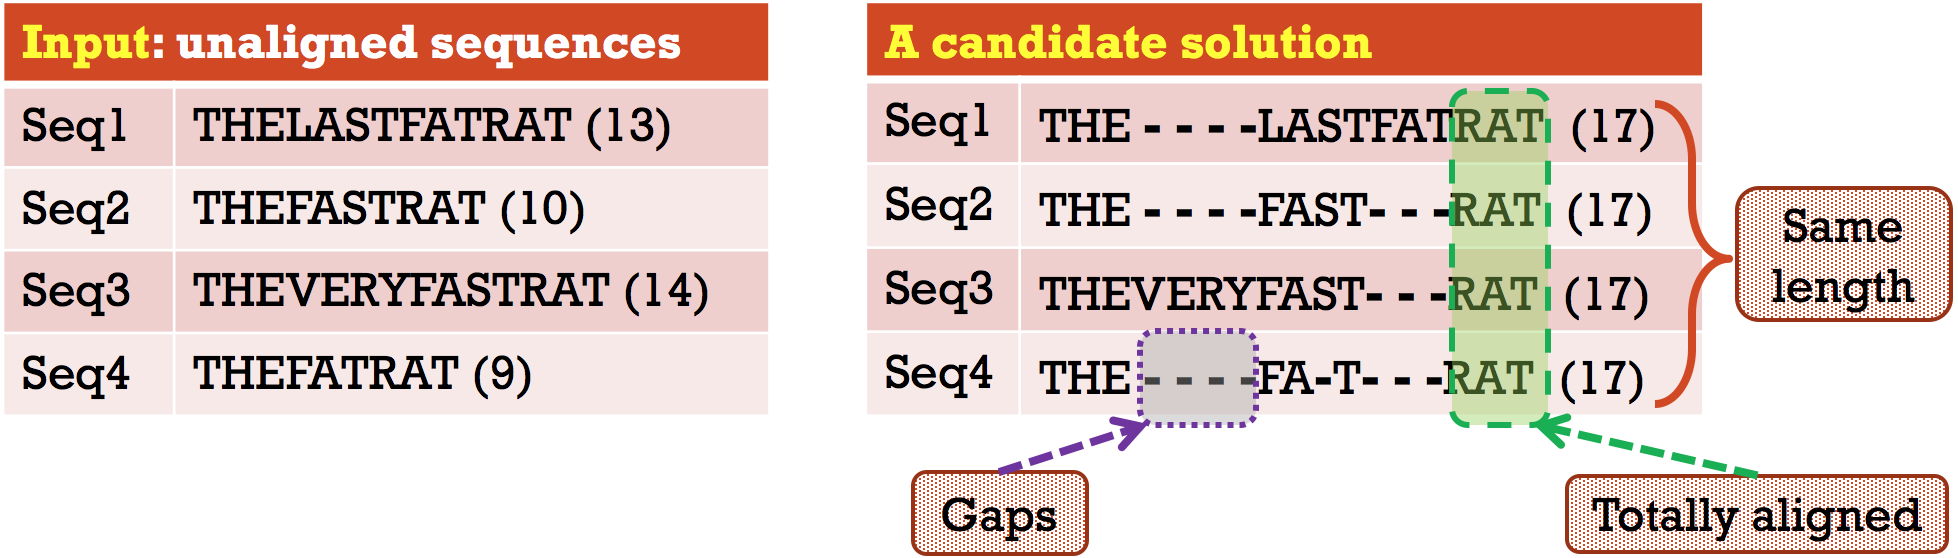
\includegraphics[width=0.8\textwidth]{cybernatics/Figure/msa_io}
	\caption{A hypothetical instance of MSA task with four protein sequences.} 
	\label{fig:msa_io}
\end{figure}

\graphicspath{{cybernatics/supp/}}

% Table generated by Excel2LaTeX from sheet 'acronym'
\begin{table}[htbp]
	\centering
	%\begin{adjustwidth}{-0.2cm}{}
	\scriptsize
	\caption{Alphabetic list of acronyms used in this study.}
	\begin{tabular}{|L{2cm}|L{13cm}|}
		\hline
		\multicolumn{1}{|c|}{Acronym} & \multicolumn{1}{c|}{Usage} \\
		\hline
		23S.E & A biological rRNA dataset  \\
		\hline
		23S.E.aa\_ag & A biological rRNA dataset  \\
		\hline
		BBXY0MN & MN$^{th}$ BAliBASE instance under RVXY group \\
		\hline
		Clustal $\Omega$ & A state-of-the-art MSA method \\
		\hline
		Clustal W & A state-of-the-art MSA method \\
		\hline
		FN rate & False negative rate, measures quality of a phylogenetic tree w.r.t. the reference tree \\
		\hline
		FSA   & A state-of-the-art MSA method \\
		\hline
		Gap   & No. of gaps, an objective function that measures goodness of an MSA \\
		\hline
		GapCon & Concentration of gaps, an objective function that measures goodness of an MSA \\
		\hline
		Kalign & A state-of-the-art MSA method \\
		\hline
		MAFFT & A state-of-the-art MSA method \\
		\hline
		ML & Maximum likelihood approach for inferring a phylogenetic tree from an MSA\\
		\hline
		MSA   & Multiple sequence alignment \\
		\hline
		MUSCLE & A state-of-the-art MSA method \\
		\hline
		NSGA-II & A multi-objective metaheuristics  \\
		\hline
		NSGA-III & A multi-objective metaheuristics which an improved version of NSGA-II to handle more than three objective functions  \\
		\hline
		PASTA & A state-of-the-art MSA method \\
		\hline
		PRANK & A state-of-the-art MSA method \\
		\hline
		ProbCons & A state-of-the-art MSA method \\
		\hline
		R0   & A random replicate of 100-taxon simulated dataset \\
		\hline
		R14   & A random replicate of 100-taxon simulated dataset \\
		\hline
		R19   & A random replicate of 100-taxon simulated dataset \\
		\hline
		R4   & A random replicate of 100-taxon simulated dataset \\
		\hline
		R9   & A random replicate of 100-taxon simulated dataset \\
		\hline
		RetAlign & A state-of-the-art MSA method \\
		\hline
		RV11  & One of the six groups of BAliBASE 3.0 benchmark \\
		\hline
		RV12  & One of the six groups of BAliBASE 3.0 benchmark \\
		\hline
		RV20  & One of the six groups of BAliBASE 3.0 benchmark \\
		\hline
		RV30  & One of the six groups of BAliBASE 3.0 benchmark \\
		\hline
		RV40  & One of the six groups of BAliBASE 3.0 benchmark \\
		\hline
		RV50  & One of the six groups of BAliBASE 3.0 benchmark \\
		\hline
		SimG  & Similarity based on gap columns, an objective function that measures goodness of an MSA \\
		\hline
		SimNG & similarity based on non-gap columns, an objective function that measures goodness of an MSA \\
		\hline
		SOP   & Sum of pairs, an objective function that measures goodness of an MSA without using the reference alignment\\
		\hline
		SP score & Sum-of-pair score, measures quality of an MSA w.r.t. the reference alignment  \\
		\hline
		T-Coffee & A state-of-the-art MSA methods \\
		\hline
		TC & No. of totally aligned columns, an objective function that measures goodness of an MSA without using the reference alignment \\
		\hline
		TC score & Total-column score, measures quality of an MSA w.r.t. the reference alignment  \\
		\hline
		wSOP  & Weighted sum of pairs, an objective function that measures goodness of an MSA \\
		\hline
	\end{tabular}%
	\label{tab:acronyms}%
	%\end{adjustwidth}
\end{table}%

\section{Objective functions for MSA}
\label{sec:objective _function}
There are numerous objective functions defined for MSA in the literature. We identify the following widely used objective functions from the recent works and briefly discuss their feasibility in MSA:

\begin{itemize}
	
	\item \textbf{Maximize sum of pairs score}~\cite{seeluangsawat2005multiple, da2010alineaga}:  
	This is an extension of pairwise sequence alignment score. Pairwise score is calculated for each pair of aligned sequences. Then, we calculate the total score by summing pairwise scores of all possible pairs. In Figure \ref{fig:pairwise}, the pairwise score is calculated by considering the elements of the same columns of two aligned sequences with the scoring or substitution matrix $\delta$. There are some standard substitution matrices for biological sequences at~\url{ftp://ftp.ncbi.nih.gov/blast/matrices/}.
	
	
	\begin{figure}[!htbp]
		\begin{adjustwidth}{-0.2cm}{}
			\centering
			\begin{subfigure}[b]{0.5\columnwidth}
				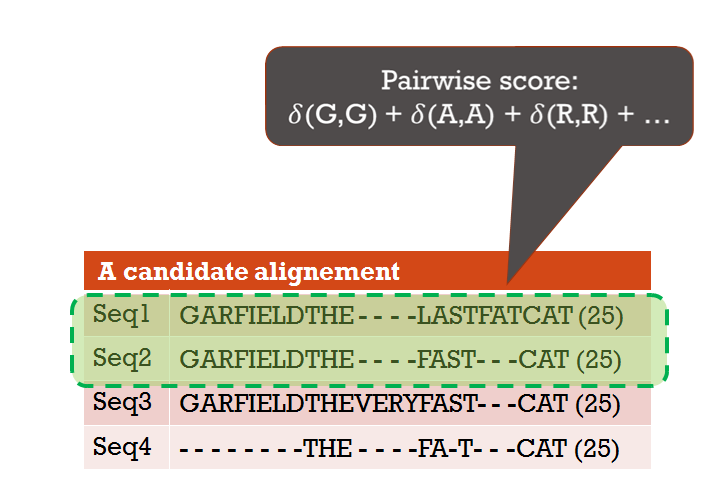
\includegraphics[width=\columnwidth]{Figure/pairwise}
				\caption{Pairwise score of two aligned sequences.}
				\label{fig:pairwise}
			\end{subfigure}	
			\begin{subfigure}[b]{0.5\columnwidth}
				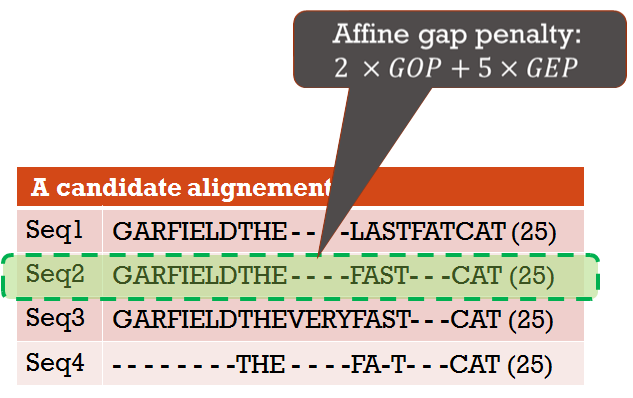
\includegraphics[width=\columnwidth]{Figure/agp}
				\caption{Affine gap penalty of an aligned sequence.}
				\label{fig:agp}
			\end{subfigure}
			\begin{subfigure}[b]{0.5\columnwidth}
				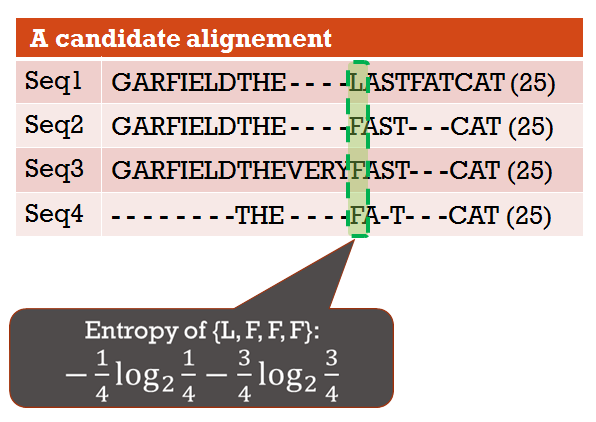
\includegraphics[width=\columnwidth]{Figure/entropy_score}
				\caption{Entropy of a column of alignment.}
				\label{fig:entropy}
			\end{subfigure}
		\end{adjustwidth}
		\caption{Three objective functions for MSA. The example alignment is adopted from~\citep{rubio2016hybrid}.}
		\label{fig:msa_obj}
	\end{figure}
	
	\item \textbf{Minimize entropy}~\cite{soto2014multi}: 
	Entropy is a measurement of dissimilarity in the same columns of different aligned sequences. When all the columns contain same element, the entropy is minimum \(0\). Again, the entropy is maximum \(1\) when every element is different. Total entropy is calculated by summing up entropy values of all columns. Figure \ref{fig:entropy} demonstrates the calculation of entropy for a single column. The problem with this function is that, while calculating entropy researchers treat gap as a separate character without proper justification.
	
	\item \textbf{Minimize affine gap penalty}~\cite{seeluangsawat2005multiple, kaya2014multiple, zhu2016novel, rani2016multiple}: 
	Affine gap penalty assigns different penalty for opening a gap ($GapOpeningPenalty, GOP$) and extending a gap ($GapExtension\-Penaly, GEP$) while computing gap penalty for a particular sequence. Then finally, summation of gap penalties of all sequences is to be minimized. An example is demonstrated in Figure \ref{fig:agp} showing the calculation of gap penalty of one sequence. Here two ideas (i.e. percentage of gap and concentration of gap) are combined without explanation. Also researchers face trouble to fix the value of two penalties.
	
	\item \textbf{Maximize weighted sum of pairs score with affine gap penalties}~\cite{rubio2016hybrid, rubio2016bee}:  
	Here two objectives are combined in the form: weighted sum of pairs score - affine gap penalty. To calculate weighted sum of pairs score, score of each pair of characters are multiplied by the sequence weight between that the corresponding two sequences. This weight is computed using the Levenshtein distance between two non-aligned sequences. Levenshtein distance is the is the minimum number of insertions, deletions or substitutions needed to convert one sequence into the other. 
	
	\item \textbf{Maximize number of totally aligned columns}~\cite{ortuno2013optimizing, da2010alineaga, rubio2016hybrid, rubio2016bee, ortuno2013optimizing, zambrano2017comparing}:
	Maximizing the number of totally aligned columns is the most simple used objective. But for input data comprising large number of taxa, its value is confined to a few values.
	
	\item \textbf{Minimize percentage of gaps}~\cite{abbasi2015local, ortuno2013optimizing, zambrano2017comparing}:
	High percentage of gaps means the sequences had to be significantly modified to align with each other. This is used as a minimizing objective function to find a better candidate solution. It can be also considered as percentage of non-gaps.
	
	\item \textbf{Maximize similarity}~\cite{kaya2014multiple, rani2016multiple}:
	%Similarity performs a measure of structural similarity among all sequences defining an individual. 
	For each column of MSA, similarity considers the ratio of the dominant character. This ratio is averaged over all columns. The closer the value of similarity is to one, the larger the probability that the candidate alignment will be discovered as the best possible alignment. Here we find similar problem as with entropy. Researchers discard gap while calculating ratio of characters in a column without sound reasoning. 
	
\end{itemize}

%\section{Multi-objective optimization}
\section{Multi-objective metaheuristics}
\label{sec:mop}
While optimizing multiple objective functions simultaneously, a multi-objective metaheuristics determines a set of solutions (instead of a single solution) which represents the best-possible compromise of all objectives. A solution is said to dominate another one if and only if it is equal to that solution in all objectives and also better than that in at least one objective. A solution is said to be Pareto optimal if no other solutions can dominate it. The set of all Pareto optimal solutions is called Pareto set and the image of pareto set in the objective space is known as Pareto front. However, practically a multi-objective metaheuristics aims to approximate the Pareto front as precisely as possible with a finite number of solutions.

%\subsection{Evolutionary algorithms}
Among metaheuristics, multi-objective evolutionary algorithms (MOEAs) are well-suited to solve multi-objective optimization problems~\cite{yang2013grid}. MOEAs deal with a set of possible solutions (known as population) at once which allows finding several members of the Pareto front in a single run of the algorithm. Moreover, they are  black-box optimization methods which do not need particular assumptions like continuity or differentiability of the decision space. 

%So the goal of a multi-objective metaheuristics is to output a set of solutions instead of a single solution., evolutionary algorithms (EAs) are population-based, They are well suited for multi-objective optimization. 

\begin{algorithm}[!htb]
	\caption{A General structure of MOEA}
	\begin{algorithmic}[1]\label{alg:MaOEA}
		\STATE{Randomly generate the initial population $ P_0 $}
		\STATE{Evaluate the objective functions of each individual in $ P_0 $}
		\STATE{$t \leftarrow 0$}
		\WHILE{$t <$ maximum value of $t$} 
		\STATE{Generate offspring population $ Q_t $ by applying \textit{Crossover} and \textit{Mutation} on $ P_t $}
		\STATE{Evaluate the objective functions of each individual in $ Q_t $}
		\STATE{Produce generation $ P_{t+1} $ from $ P_t $ and $ Q_t $ using \textit{Ranking scheme}}
		\STATE{$t \leftarrow t + 1$ }
		\ENDWHILE
	\end{algorithmic}
\end{algorithm}

A general structure of MOEAs is summarized in Algorithm \ref{alg:MaOEA}. Here the \textit{Crossover} and \textit{Mutation} are popularly known as genetic operators. They generate offspring (new solutions) from parents (existing solutions). These are problem-specific and designed based on the actual problem to be solved. \textit{Ranking scheme} is used to choose appropriate solutions to form the next generation. This is problem-independent concept and provided by the developers of a specific algorithm. In this study, we considered the three widely used MOEAs for multi-objective optimization. We briefly describe them as follows.

\begin{enumerate}[label=(\alph*)]
	
	\item NSGA-II~\citep{deb2002fast} follows the classical structure of a generational genetic algorithm. At first, it applies the typical genetic operators (selection, crossover, and mutation) on the current population to fill an auxiliary population. Then it builds the next-generation by incorporating the best individuals from both the current and auxiliary populations according to a Pareto ranking and the crowding distance operator. Perhaps it is the most commonly used algorithm for solving optimization problems having two or three objective functions. 
	
	\item NSGA-III~\citep{deb2014evolutionary} is designed to handle a large number of objective functions. The skeleton of NSGA-III remains similar to its predecessor NSGA-II with notable changes in its selection mechanism. At each generation, it produces an offspring population from the current population by applying genetic operators. These two populations are merged to form a new population using the selection mechanism. NSGA-III continues to use Pareto dominance as the primary selection criterion to promote convergence. But it substitutes the crowding distance operator in NSGA-II with a clustering operator aided by a set of well-distributed reference points as the secondary selection criterion to maintain diversity. NSGA-III has been shown to perform reasonably.
	%NSGAIII has been shown to perform reasonably on handling a large number of objective functions~\cite{deb2014evolutionary}.
	
	\item MOEA/D~\citep{zhang2007moea} is a representative decomposition based MOEA. Unlike Pareto dominance based methods (e.g., NSGA-II, NSGA-III), It decomposes the original problem into many single-objective subproblems using an aggregation function and a series of weight vectors defining the relative importance of different objectives. %We use the Das and Dennis's procedure~\cite{das1998normal} for generating uniform weight vectors, which are evenly distributed along the 7-dimensional unit hyper-plane. 
	Then it deals with these subproblems in a collaborative manner. Neighborhood relations among these subproblems are defined based on the similarity between their weight vectors. 
	%When optimizing a subproblem, the local information from its neighboring subproblems is shared. 
	Each subproblem maintains an individual which could be the best individual found so far for it. The algorithm generates a new individual for each subproblem by performing genetic operators on some of its neighboring individuals. The current individual of both the considered subproblem and its neighbors will be updated if the new individual is better than their current one. %The procedure of MOEA/D for TNDP is presented in Algorithm~\ref{alg:moead}.	(i.e., the individuals of its neighboring subproblems) that combines all objectives
	For MSA, we adopt the MOEA/D configuration used by~\citep{zhu2015novel}.  
\end{enumerate} 



%\subsection{Our multi-objective metaheuristic framework}
%\label{sec:mof}
% Table generated by Excel2LaTeX from sheet 'multi-pc'

\begin{comment}
\subsubsection{Solution Initialization}
Instead of initializing solutions randomly, which is the usual practice in metaheuristics, we seed the initial population with alignments generated by nine state-of-the-art MSA tools. These tools are listed in Table~\ref{tab:msa_tools}. We create the required number of initial solutions by randomly mixing and modifying those nine alignments. 
%Among these tools PASTA is the most recently developed. Due to its simultaneous estimation of alignment and phylogenetic tree, it is expected to be the most robust.

\begin{table*}[htbp]
\small
\centering
\caption{List of state-of-the-art MSA tools that we used initialize the metaheuristics.}
\begin{tabular}{|l|l||l|l|}
\hline
\multicolumn{2}{|c||}{For nucleotide sequences} & \multicolumn{2}{c|}{For protein sequences} \\
\hline
\multicolumn{1}{|c|}{Tool} & \multicolumn{1}{c||}{Version} & \multicolumn{1}{c|}{Tool} & \multicolumn{1}{c|}{Version} \\
\hline
FSA~\citep{bradley2009fast} & 1.15.9 & FSA   & 1.15.9 \\
\hline
PASTA~\citep{mirarab2015pasta} & 1.7.8 & PASTA & 1.7.8 \\
\hline
T-Coffee~\citep{notredame2000t} & 11.00 & T-Coffee & 11.00 \\
\hline
MAFFT~\citep{katoh2002mafft} & 7.31  & MAFFT & 7.245 \\
\hline
Clustal W~\citep{thompson1994clustal} & 2.1   & Clustal W & 2.1 \\
\hline
Clustal $ \Omega $~\citep{sievers2011fast} & 1.2.4 & RetAlign~\citep{szabo2010reticular} & 1.0 \\
\hline
MUSCLE~\citep{edgar2004muscle} & 3.8.31 & MUSCLE & 3.8.31 \\
\hline
PRANK~\citep{loytynoja2005algorithm} & 0.170427 & ProbCons~\citep{do2005probcons} & 1.12 \\
\hline
Kalign~\citep{lassmann2008kalign2} & 2.03  & Kalign & 2.04 \\
\hline
\end{tabular}%
\label{tab:msa_tools}%
\end{table*}%

\subsubsection{Genetic Operator}
Both of our metaheuristics used the same genetic operator (i.e. mutation and crossover), which were used by~\citealp{ortuno2013optimizing}. \citealp{zambrano2017multi} illustrated their functions. Here we provide a short description of these operators. 

The mutation operator is termed as closed gap shifting, where consecutive gaps are randomly chosen and shifted to another random position in a sequence. This shifting may result columns having only gaps which are then removed. Thus this mutation tries to reduce the number of gaps in the MSA.

The crossover operator is the single-point crossover over alignments proposed by~\citealp{da2010alineaga}. The operator randomly selects a column from one parent to split it into two blocks (let us refer to them P1a and P1b). The same selected positions are located in the other parent (which are not necessarily in the same column) and is tailored so that the right piece can be joined to the left piece of the first parent and vice versa (P2a and P2b). Finally, the selected blocks are exchanged between these two parents to create two new individuals with the combination of the blocks: [P1a + P2b] and [P1a + P1b]. After that, any empty space that appears at the junction point is filled with gaps.
%\subsubsection{Multi-objective evolutionary algorithm}
%\subsubsection{Parameter Configuration}
\end{comment}

\begin{comment}


\section{Evaluation of estimated alignments}
\label{sec:msa_eval}
We evaluate estimated alignments with respect to reference alignment using two well-known alignment quality scores called TC score and SP score. These two scores are defined below:
\begin{itemize}
	\item TC score is the ratio of the number of correctly aligned columns in the estimated alignment to the total number of aligned columns in the reference alignment. This is also known as column score.
	
	\item SP score is the ratio of the number of aligned pairs in the estimated alignment to the total number of aligned pairs in the reference alignment.
	
	%\item Pairs score is the mean of SP-score and Modeler. SP-Score is the ratio of the number of aligned pairs to the total number of aligned pairs in the reference alignment. And Modeler is very similar to the SP-score where we take the ratio of the number of aligned pairs to the total number of aligned pairs in the estimated alignment  	
\end{itemize}
For both the measures, higher value implies better score.

\section{Phylogenetic tree estimation}
\label{sec:tree_estimation}
For each of the generated alignment we estimate the phylogenetic tree using Maximum Likelihood (ML) method which is the standard way of estimating phylogenetic tree from sequence data~\cite{liu2011raxml}. FastTree\citep{price2010fasttree} and RAxML~\citep{stamatakis2014raxml} are the most widely used software for this purpose. FastTree can produce output very quickly with little (and in some cases no) degradation in tree accuracy, as compared to RAxML~\cite{liu2011raxml}. In this study we had to estimate a large number of phylogenetic trees. So we choose FastTree over RAxML.
%We used a popular tool named FastTree-2 developed by \citep{price2010fasttree}. %It is publicly available at \url{http://www.microbesonline.org/fasttree/}.

\section{Evaluation of phylogenetic tree}
\label{sec:tree_eval}
We evaluate the quality of each estimated ML tree with respect to the true phylogenetic tree using a widely used measure known as the False Negative (FN) rate. FN rate is the percentage of edges present in the true tree but missing in the estimated tree. So a small value of FN rate is desirable. Although there are two more common tree error measures (False Positive (FP rate) and and Robinson-Foulds (RF) rate), all of them are identical when true and estimated trees are binary~\citep{warnow2017computational}. In this study we worked with binary trees only. %as a quality measure, 

\section{Evaluation of objective functions}
\label{sec:obj_eval}
In the context of phylogeny estimation, a desired objective function for MSA should lead to such alignments which can produce highly accurate (having small FN rate) ML trees. Considering this fact, we try to evaluate the effectiveness of an objective function by studying how its values are associated with the corresponding FN rates. The objective function that frequently exhibits positive correlation with FN rate is predicted to be a good optimization criteria. To accomplish this, we fit multiple linear regression model to calculate the degree of association (i.e., regression coefficient) between an objective and FN rate. Then we apply t-test, with null hypothesis that there is no association, to check the significance of individual regression coefficients. It should be noted that, such regression results does not necessarily indicate the strength of an objective as an optimization criterion. However, such results can definitely be utilized as the starting point for experimentation for further validation.

\end{comment} 
